\documentclass{article}
\usepackage[%
    left=0.5in,%
    right=0.5in,%
    top=0.5in,%
    bottom=0.5in,%
]{geometry}%
\usepackage{minitoc}
\usepackage{multicol}
\usepackage{graphicx}
\usepackage{fixltx2e}
\usepackage{hyperref}
\usepackage{hyperref}
    \hypersetup{ colorlinks = true, linkcolor = blue }
\usepackage{blindtext}

\graphicspath{ {./} }

\newcommand{\inlinecode}[2]{\colorbox{lightgray}{\lstinline
[language=#1]$#2$}}
\newcommand{\worddef}[1]{\hyperref[sec:reference]{\textit{#1}}}

\begin{document}

\section{Paging}
\subsection{Address translation: implementation}
\begin{flushleft}
A logical (physical) address is \textbf{relative} to the start of the program (memory) and consists of two parts:
\begin{itemize}
	\item The \textbf{left} most n bits that represent the page (frame) \textbf{number} e.g. 4 bits for the page number allowing 16 (24 ) pages (frames)
	\item  The \textbf{right} most m bits that represent the \textbf{offset} within the page (frame) e.g. 12 bits for the offset, allowing up to 4096 (212) bytes per page (frame)
\end{itemize}
 The offset within the page and frame remains the same (\textbf{they are the same size}). The page number to frame number \textbf{mapping} is held in the \textit{page table}.
\begin{center}
	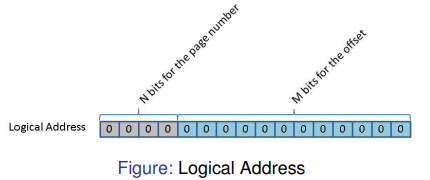
\includegraphics[scale=0.6]{logical_address.png}
\end{center}
\bigskip
Steps in address translation:
\begin{itemize}
	\item Extract the page number from logical address
	\item Use page number as an index to retrieve the frame number in the page table
	\item Add the “logical offset within the page” to the start of the physical frame
\end{itemize}
\textbf{Hardware} implementation of address translation
\begin{itemize}
	\item The CPU’s memory management unit (MMU) intercepts logical addresses
	\item MMU uses a page table as above
	\item The resulting physical address is put on the memory bus
\end{itemize}
\end{flushleft}

\subsection{Entry contents}
\begin{itemize}
	\item A \textbf{“present/absent bit”} that is set if the page/frame is in memory
	\item A \textbf{“modified bit”} that is set if the page/frame has been modified (\textbf{only modified pages} have to be written back to disk when evicted)
	\item A \textbf{“referenced bit”} that is set if the page is in use
	\item \textbf{Protection and sharing bits}: read, write, execute or combinations thereof
\end{itemize}
\begin{center}
	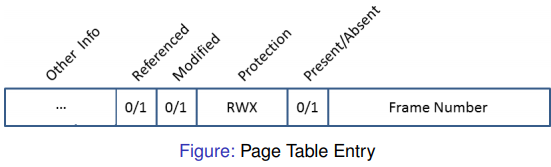
\includegraphics[scale=0.6]{page_table_entry.png}
\end{center}

\subsection{Dealing with large page tables}
\begin{flushleft}
How do we deal with the increasing size of page tables, i.e., where do we store them?
\begin{itemize}
	\item Their size \textbf{prevents} them from being stored in registers.
	\item They have to be stored in (\textbf{virtual}) main memory:
	\begin{itemize}
		\item \textbf{Multi-level} page tables.
		\item \textbf{Inverted} page tables (for \textbf{large} virtual address spaces)
	\end{itemize}
	\item How can we maintain acceptable speeds?: address translation happens at every memory reference, it has to be fast!
	\item Accessing main memory results in memory stalls
\end{itemize}
\bigskip
Solution: \textbf{Page} the \textit{page table}!
\begin{itemize}
	\item We keep tree-like structures to hold page tables
	\item Divide the page number into
	\begin{itemize}
		\item An index to a page table of second level
		\item A page within a second level page table
	\end{itemize}	
	\item No need to keep all page tables in memory all time
\end{itemize}
\textbf{Memory organisation} of multi-level page tables:
\begin{itemize}
	\item The root page table is \textbf{always} maintained in \textbf{memory}
	\item Page tables themselves are maintained in \worddef{virtual memory} due to their \textbf{size}
\end{itemize}
\end{flushleft}

\section{Virtual memory}
\subsection{Locality}
\begin{flushleft}
Are there any other benefits of \textit{paging}?
\begin{itemize}
	\item Code execution and data manipulation are usually restricted to a \textbf{small subset} (i.e. limited number of pages) at any point in time I.e. code and data references within a process are usually \textbf{clustered}. This is called the \textit{principle of locality}.
	\item Not all pages have to be loaded in memory at the same time ⇒ virtual memory
\end{itemize}
Loading an entire set of pages for an entire program/data set into memory is \textbf{wasteful}. Desired blocks could be loaded on demand
\end{flushleft}

\subsection{Page faults}
\begin{flushleft}
The \textit{resident set} refers to the pages that are loaded in main memory.A \textit{page fault} is generated if the processor accesses a page that is not in memory.
\begin{itemize}
	\item A page fault results in an \textbf{interrupt} (process enters blocked state).
	\item An I/O operation is started to \textbf{bring the missing page into} main memory.
	\item A \textit{context switch} (may) take place
	\item \textbf{An interrupt} signals that the I/O operation is complete (process enters \textit{ready state})
\end{itemize}
\end{flushleft}

\subsubsection{Processing page faults}
\begin{itemize}
	\item Trap operating system
	\begin{itemize}
		\item Save registers/process state
		\item Analyse interrupt (i.e., identify page fault)
		\item Validate page reference, determine page location
		\item Issue disk I/O: queueing, seek, latency, transfer
	\end{itemize}
	\item Context switch (optional)
	\item Interrupt for I/O completion
	\begin{itemize}
		\item Store process state/registers
		\item Analyse interrupt from disk
		\item Update page table (page in memory)
		\item Wait for original process to be scheduled
	\end{itemize}
	\item Context switch to original process
\end{itemize}

\subsection{Benefits}
\begin{flushleft}
Being able to maintain more processes in main memory through the use of virtual memory \textbf{improves} CPU utilisation.
\begin{itemize}
	\item Individual processes take up \textbf{less} memory since they are only \textbf{partially loaded}
	\item Virtual memory allows the \textit{logical address space} (i.e processes) to be \textbf{larger} than \textit{physical address space} (i.e. main memory) 64 bit machine \verb!⇒ ! $2^{64}$ logical addresses (theoretically)
\end{itemize}
\end{flushleft}

\pagebreak
\section*{Reference section} \label{sec:reference}
\begin{description}
	\item[virtual memory] \hfill \\ a storage area that holds the files on your hard drive for retrieval when a computer runs out of RAM.
\end{description}
\end{document}
